\chapter{Evaluace zpětné vazby od ostatních studentů VŠE}\label{chap:zpetna-vazba}

Tato kapitola se zabývá evaluací zpětné vazby od ostatních studentů Vysoké školy ekonomické v~Praze, která byla sesbírána pomocí metody dotazníkového šetření. Kapitola obsahuje proces za návrhem dotazníku

Pro sběr zpětné vazby od ostatních studentů Vysoké školy ekonomické v~Praze pro následnou evaluaci byla zvolena metoda dotazníkového šetření. Cílem dotazníku je lépe pochopit potřeby uživatelů webového rozšíření a zodpovědět stanovené hypotézy.

Byly stanoveny následující hypotézy, které jsou se dotazníkové šetření:

\begin{enumerate}
    \item Většina uživatelů rozšíření využívá rozšíření s~přihlášením.
    \item Většina uživatelů rozšíření využívá alespoň 2 z~přidaných funkcionalit.
    \item Výsledky dotazníkového šetření odpovídají počáteční analýze používání systému InSIS.
\end{enumerate}

\section{Návrh dotazníku}

Dotazník byl vytvořen prostřednictvím platformy Google Forms, která umožňuje jednoduchou editaci a zároveň poskytuje nástroje pro tvorbu komplexních dotazníků, jako větvení průchodu dotazníkem podle předchozích odpovědí respondenta. To je užitečné například pro zobrazení odlišných otázek respondentům, kteří rozšíření nepoužívají, aby byla zpětná vazba co nejrelevantnější. Nedávalo by smysl se respondentů, kteří rozšíření nepoužívají ptát na dílčí funkcionality nebo se naopak dotazovat uživatelů, kteří rozšíření mají nainstalované, jaké jsou jejich primární důvody proč rozšíření nepoužívají. 

Celý dotazník je členěn do 8 sekcí, které se respondentům zobrazují v~závislosti na předchozích odpovědích. Každá část dotazníku obsahuje 1-20 otázek, které jsou buď výběr 1 nebo více možností z~předem stanoveného výběru nebo otevřené odpovědi s~doplněním vlastního textu. Schéma průchodu dotazníkem zobrazuje obrázek \ref{fig:dotaznik}.

\begin{figure}[htbp!]\centering
    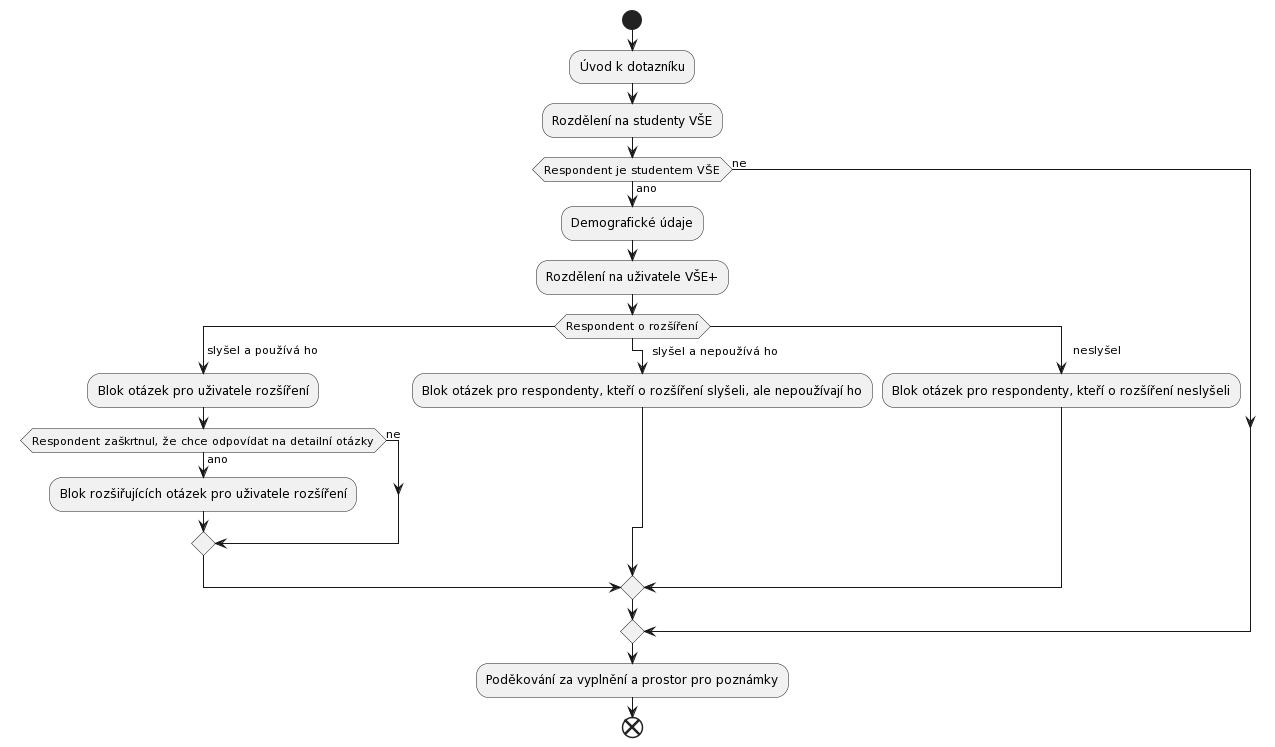
\includegraphics[width=\textwidth]{img/dotaznik.png}
    \caption{Schéma průchodu dotazníkem (vlastní zpracování)}
    \label{fig:dotaznik}
\end{figure}
\imagesource{
@startuml
start
:Úvod k~dotazníku;

:Rozdělení na studenty VŠE;

if (Respondent je studentem VŠE) then (ano)
  :Demografické údaje;
  :Rozdělení na uživatele VŠE+;
  switch (Respondent o~rozšíření) 
  case ( slyšel a používá ho) 
    :Blok otázek pro uživatele rozšíření;
    if (Respondent zaškrtnul, že chce odpovídat na detailní otázky) then (ano)
        :Blok rozšiřujících otázek pro uživatele rozšíření;
    else (ne)
    endif
  case (     slyšel a nepoužívá ho)
    :Blok otázek pro respondenty, kteří o~rozšíření slyšeli, ale nepoužívají ho;
  case (   neslyšel)
    :Blok otázek pro respondenty, kteří o~rozšíření neslyšeli;
  endswitch
else (ne)
endif

:Poděkování za vyplnění a prostor pro poznámky;
end
@enduml
}

\section{Představení dat}

Celkem bylo v~dotazníkovém šetření nasbíráno od respondentů 85 odpovědí. Z~tohoto celku je 74 odpovědí od respondentů, kteří jsou v~současné době studenty Vysoké školy ekonomické v~Praze a o~rozšíření VŠE+ slyšeli. Z~těchto 74 odpovědí pak 42 respondentů chtělo odpovídat na doplňující otázky ke každé z~implementovaných funkcionalit. Vzhledem k~počtu instalací webového rozšíření se jedná o~poměrně rozsáhlý vzorek uživatelů. 

\subsection{Demografie respondentů}

Jako relevantní demografické údaje sbírané od respondentů byly zvoleny údaje o~stupni vysokoškolského studia, ročníku a fakultě, na které respondent studuje. Z~celkového počtu 74 respondentů bylo 71 respondentů z~fakulty informatiky a statistiky, což je pravděpodobným důsledkem zvolených způsobů sdílení formuláře.

Rozložení počtu respondentů vzhledem k~stupni vysokoškolského studia a ročníku je možné vidět na obrázku \ref{fig:demografie-respondentu}. Nejpočetnější skupinou respondentů v~tomto zobrazení jsou studenti 3. ročníku bakalářských studií, což může být opět důsledkem zvoleného způsobu sdílení formuláře. Zajímavým jevem, který je možné vypozorovat na obrázku \ref{fig:zdroj-instalace} je skutečnost, že studenti prvních a druhých ročníků se v~porovnání se studenty třetích ročníků o~rozšíření častěji dozvěděli z~doporučení od spolužáka, zatímco studenti třetích ročníků se nejčastěji o~rozšíření dozvěděli prostřednictvím neoficiálního fakultního serveru na chatovací platformě Discord. 

\begin{figure}[htbp!]\centering
    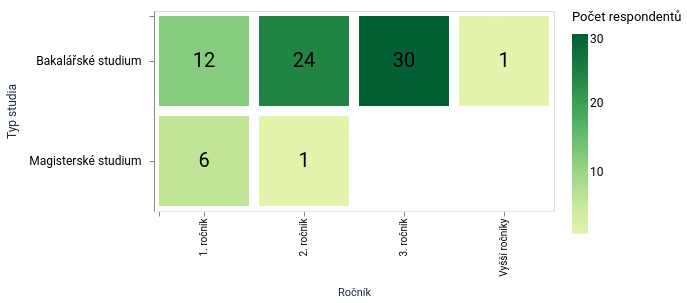
\includegraphics[width=\textwidth]{img/demografie-respondentu.png}
    \caption{Demografie respondentů dotazníkového šetření (vlastní zpracování)}
    \label{fig:demografie-respondentu}
\end{figure}

\begin{figure}[htbp!]\centering
    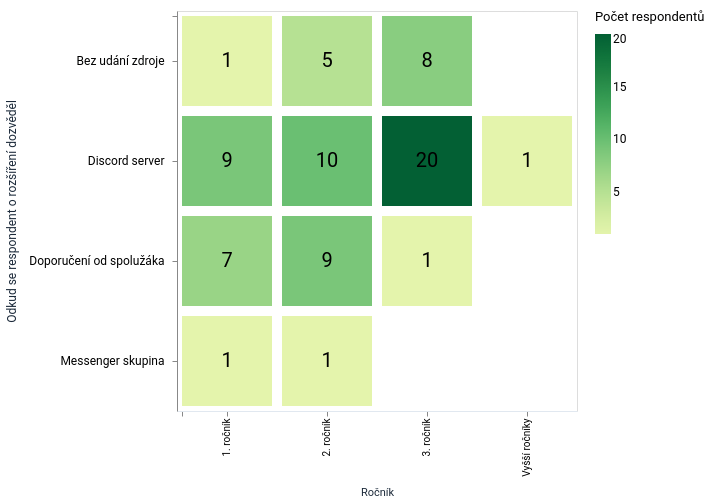
\includegraphics[width=\textwidth]{img/zdroj-instalace.png}
    \caption{Zdroje, ze kterých se respondenti o~rozšíření dozvěděli (vlastní zpracování)}
    \label{fig:zdroj-instalace}
\end{figure}

\subsection{Využívání přidaných funkcionalit}

Ve čtvrté sekci dotazníku všichni respondenti, kteří jsou současnými nebo bývalými studenty VŠE vybírali z~výběru 1 nebo více přidaných funkcionalit, které používají. Nasbírané statistiky od 60 respondentů zobrazuje graf na obrázku \ref{fig:features-data}. 51 respondentů využívá funkcionalitu náhledu rozvrhu při registraci rozvrhových akcí, 38 respondentů využívá funkcionalitu připomínání odevzdáváren a 52 respondentů využívá funkcionalitu vylepšeného rozvrhu. 

\begin{figure}[htbp!]\centering
    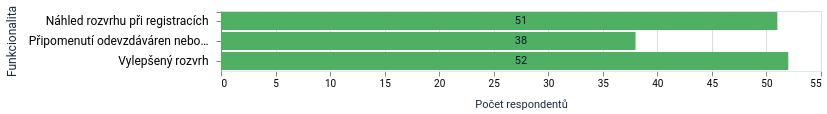
\includegraphics[width=\textwidth]{img/features.png}
    \caption{Statistiky využívání přidaných funkcionalit (vlastní zpracování)}
    \label{fig:features-data}
\end{figure}

\subsection{Evaluace zpětné vazby k~implementaci vylepšeného rozvrhu}

V~sekci dotazníku zaměřené na modul s~vylepšeným rozvrhem byly na respondenty kladeny 3 otázky týkající se využívání dílčích funkcionalit pro lepší pochopení interakce respondentů s~rozvrhem. Jak zobrazuje obrázek \ref{fig:timetable-feedback}, na otázku jestli respondenti využívají možnosti přepínání mezi jednotlivými týdny ve výukovém období 24 respondentů odpovědělo že ano a 18 respondentů odpovědělo že ne. Na otázku jestli respondenti využívají možnosti přidávání poznámek k~hodinám v~rozvrhu odpovědělo 6 respondentů ano a 36 respondentů ne. 

Toto bylo pro autora překvapivé zjištění, protože na základě analýzy práce s~rozvrhem studentů předcházející samotné implementaci rozšíření vyplynulo, že ostatní studenti mají podobný workflow práce s~rozvrhem jako autor. Výsledky dotazníkového šetření ovšem tento předpoklad vyvrací a potvrzují alternativní hypotézu, že se chování ostatních uživatelů rozšíření liší od výsledku analýzy.

\begin{figure}[htbp!]\centering
    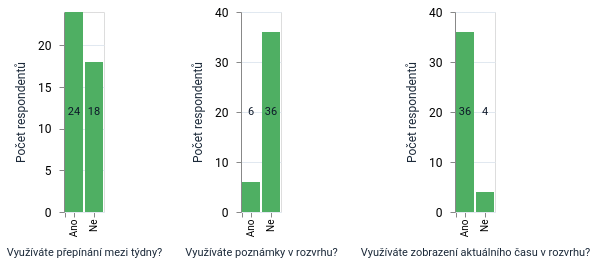
\includegraphics[width=\textwidth]{img/timetable.png}
    \caption{Využití dílčích částí vylepšeného rozvrhu (vlastní zpracování)}
    \label{fig:timetable-feedback}
\end{figure}

\subsection{Evaluace zpětné vazby k~implementaci připomenutí odevzdáváren}


V~sekci dotazníku se zpětnou vazbou k~implementaci připomínání odevzdáváren byly respondentům dotazníku kladeny 3 kvantitativní otázky. Tyto otázky byly definovány následovně:

\begin{enumerate}
    \item Využíváte možnost nechat si na odevzdávárny zaslat upozornění?
    \item Využíváte možnost exportovat odevzdávárny do Google kalendáře / Outlooku?
    \item Vyhovuje vám výběr časů před uzavřením odevzdávárny?
\end{enumerate}

Na každou z~otázek respondenti odpovídali buď ano nebo ne s~výjimkou 3. z~uvedených otázek, kde byla přidána do výběru možnost, že připomínání odevzdáváren respondent nevyužívá.

Kromě těchto 3 kvantitativních otázek byly v~této sekci definovány i 3 kvalitativní otázky, ve kterých respondenti odpovídali, jestli používají jiné platformy pro správu kalendáře kromě dvou již podporovaných platforem, jestli existuje nějaká skutečnost, která jim na implementaci této funkcionality vadí, a jestli jim naopak něco v~implementaci chybí.

\begin{figure}[htbp!]\centering
    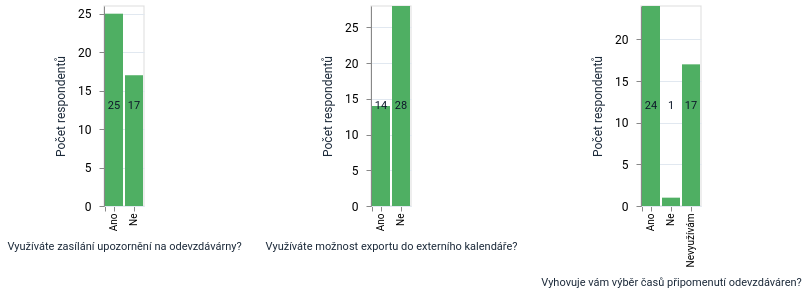
\includegraphics[width=\textwidth]{img/pripomenuti-vizualizace.png}
    \caption{Využití dílčích částí připomenutí odevzdáváren (vlastní zpracování)}
    \label{fig:pripomenuti-vizualizace}
\end{figure}

Odpovědi respondentů v~této sekci dotazníku odpovídají počáteční analýze, protože většina studentů využívá zasílání upozornění na email a pouze menšina využívá export do externího kalendáře. Pozitivní zpětnou vazbou bylo ověření vhodného výběru časů připomenutí, které vyhovovaly 24 z~25 uživatelům rozšíření, kteří funkcionalitu připomenutí odevzdáváren využívají.

\subsection{Evaluace zpětné vazby k~náhledu rozvrhu při registracích}

V~této sekci dotazníku byly na respondenty kladeny 2 kvantitativní otázky a podobně jako u~ostatních částí na dílčí funkcionality, také 2 kvalitativní otázky.

Cílem této části dotazníku bylo zhodnotit míru využívání náhledu rozvrhu při registraci předmětů a získat zpětnou vazbu k~implementaci vyznačování hodin s~kolizí v~rozvrhu. Hlavní zmiňovanou položkou při prvotních konzultacích s~uživateli rozšíření byla grafická stránka implementace, proto byly do možných odpovědí na otázku "Pomáhá vám při registracích funkce detekcí kolizí v~rozvrhu?" přidány možnosti "Ano, ale ocenil bych možnost vypnout grafické rozlišení" a "Ano, ale změnil bych grafické rozlišení".  

\begin{figure}[htbp!]\centering
    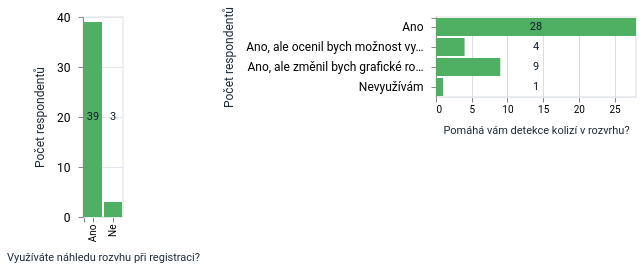
\includegraphics[width=\textwidth]{img/previews-visualization.png}
    \caption{Využití dílčích částí náhledu rozvrhů (vlastní zpracování)}
    \label{fig:pripomenuti-vizualizace}
\end{figure}

Odpovědi respondentů v~této sekci dotazníku odpovídají počáteční analýze, protože většina studentů využívá zasílání upozornění na email a pouze menšina využívá export do externího kalendáře. Pozitivní zpětnou vazbou bylo ověření vhodného výběru časů připomenutí, které vyhovovaly 24 z~25 uživatelům rozšíření, kteří funkcionalitu připomenutí odevzdáváren využívají.

\subsection{Evaluace zpětné vazby k~náhledu rozvrhu při registracích}

V~této sekci dotazníku byly na respondenty kladeny 2 kvantitativní otázky a podobně jako u~ostatních částí na dílčí funkcionality, také 2 kvalitativní otázky.

Cílem této části dotazníku bylo zhodnotit míru využívání náhledu rozvrhu při registraci předmětů a získat zpětnou vazbu k~implementaci vyznačování hodin s~kolizí v~rozvrhu. Hlavní zmiňovanou položkou při prvotních konzultacích s~uživateli rozšíření byla grafická stránka implementace, proto byly do možných odpovědí na otázku "Pomáhá vám při registracích funkce detekcí kolizí v~rozvrhu?" přidány možnosti "Ano, ale ocenil/a bych možnost vypnout grafické rozlišení" a "Ano, ale změnil/a bych grafické rozlišení".    

Graf na obrázku \ref{fig:nahledy-vizualizace} zachycuje zastoupení jednotlivých odpovědí na kvantitativní otázky.

\begin{figure}[htbp!]\centering
    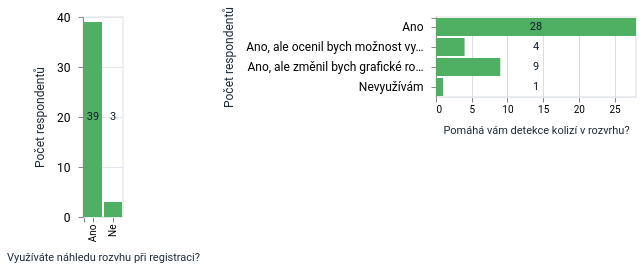
\includegraphics[width=\textwidth]{img/previews-visualization.png}
    \caption{Využití dílčích částí náhledu rozvrhů (vlastní zpracování)}
    \label{fig:nahledy-vizualizace}
\end{figure}

\section{Výsledky dotazníkového šetření}

Na základě odpovědí od respondentů dotazníkového šetření byly zodpovězeny hypotézy stanovené na začátku kapitoly.

První hypotéza "většina uživatelů rozšíření využívá rozšíření s~přihlášením" byla potvrzena, jelikož 86.7 \% respondentů, kteří odpověděli, že rozšíření používají, používá rozšíření s~aktivním přihlášením pomocí školního účtu.

Druhá hypotéza "většina uživatelů rozšíření využívá alespoň 2 z~přidaných funkcionalit" byla také potvrzena, jelikož přes 83 \% respondentů, kteří odpověděli, že rozšíření používají, používá alespoň 2 z~přidaných funkcionalit.

Poslední hypotéza "výsledky dotazníkového šetření odpovídají počáteční analýze používání systému InSIS" je jedinou hypotézou, která nebyla potvrzena. Důvodem je rozpor počáteční analýzy v~oblasti používání rozvrhu a předpokladu používání poznámek přímo v~rozvrhu a sesbíraných dat, která indikují pouze minimální využívání této přidané funkcionality. Chybná počáteční analýza používání rozvrhu mohla být způsobena velice omezeným počtem respondentů.
